\documentclass{beamer}
\usepackage[english, russian]{babel}
\usepackage[T2A]{fontenc}
\usepackage[utf8]{inputenc}
\usepackage{indentfirst}
\usepackage{amsmath, amsfonts, amssymb, amsthm, mathtools}
\usepackage[export]{adjustbox}
\usepackage{graphicx} 
\graphicspath{ {./images/} }

\usepackage{subcaption}
\usepackage{verbatim}

\usepackage{minted}{\setlength{\parskip}{0pt}}

\usepackage{hyperref}

\hypersetup{
    colorlinks=true,
    linkcolor=blue,
    filecolor=magenta,      
    urlcolor=black,
    pdftitle={Overleaf Example},
    pdfpagemode=FullScreen,
    }


\title{Отчет по лабораторной работе № 2. \\ Настройка DNS-сервера.}
\author{Данила Стариков \\ НПИбд-02-22}
\date{2024}

\begin{document}

\maketitle
\newpage

\tableofcontents

\newpage
\section{Цель работы}
Приобретение практических навыков по установке и конфигурированию DNS-сервера, усвоение принципов работы системы доменных имён.

\newpage
\section{Выполнение работы}
\subsection{Установка DNS-сервера}
\begin{enumerate}
    \item Загрузили вашу операционную систему и перейдите в рабочий каталог с проектом:
        \begin{minted}{bash}
        cd /home/tmp/dastarikov/vagrant
        \end{minted}
    \item Запустили виртуальную машину server:
        \begin{minted}{bash}
        make server-up
        \end{minted}
    \item На виртуальной машине server вошли под созданным  в предыдущей работе пользователем и открыли терминал. Перешли в режим суперпользователя:
        \begin{minted}{bash}
        sudo -i
        \end{minted}
    \item Установили bind и bind-utils:
        \begin{minted}{bash}
        dnf -y install bind bind-utils
        \end{minted}

    \item В качестве упражнения с помощью утилиты dig сделали запрос к DNS-адресу \url{www.yandex.ru} (Рис. \ref{01}):
        \begin{minted}{bash}
        dig www.yandex.ru
        \end{minted}

\begin{center}
    \centering
    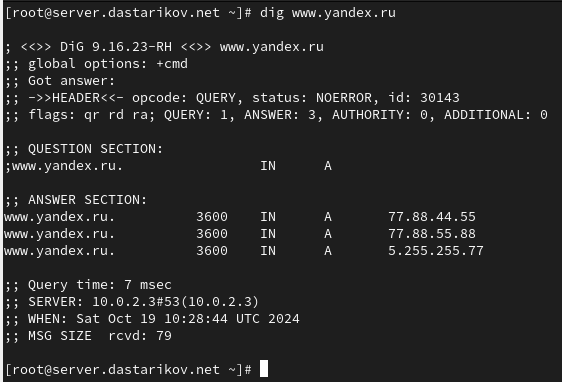
\includegraphics[width=0.8\textwidth]{../images/image01.png}
    \captionof{figure}{Запрос к DNS-адресу www.yandex.ru}
    \label{01}
\end{center}

\end{enumerate}

\subsection{Конфигурирование кэширующего DNS-сервера}
\subsubsection{Конфигурирование кэширующего DNS-сервера при отсутствии фильтрации DNS-запросов маршрутизаторами}
\begin{enumerate}
    \item Запустили DNS-сервер:
        \begin{minted}{bash}
        systemctl start named
        \end{minted}
    \item Включили запуск DNS-сервера в автозапуск при загрузке системы:
        \begin{minted}{bash}
        systemctl enable named
        \end{minted}
    \item Проанализировали в отчёте отличие в выведенной на экран информации при выполнении команд (Рис. \ref{02} и \ref{03})
        \begin{minted}{bash}
        dig www.yandex.ru
        \end{minted}

\begin{center}
    \centering
    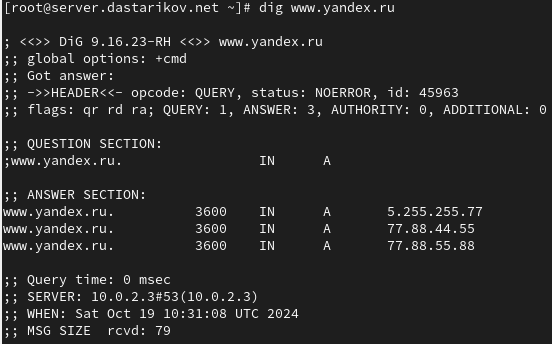
\includegraphics[width=0.8\textwidth]{../images/image02.png}
    \captionof{figure}{Запрос к DNS-адресу www.yandex.ru}
    \label{02}
\end{center}

    и
        \begin{minted}{bash}
        dig @127.0.0.1 www.yandex.ru
        \end{minted}

\begin{center}
    \centering
    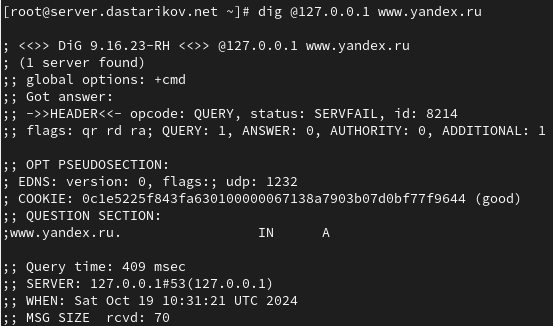
\includegraphics[width=0.8\textwidth]{../images/image03.png}
    \captionof{figure}{Запрос к DNS-адресу www.yandex.ru с заданным адресом сервера.}
    \label{03}
\end{center}

    \item Сделали DNS-сервер сервером по умолчанию для хоста server и внутренней виртуальной сети. Для этого требуется изменить настройки сетевого соединения eth0 в NetworkManager, переключив его на работу с внутренней сетью и указав для него в качестве DNS-сервера по умолчанию адрес 127.0.0.1 (Рис. \ref{04}):
        \begin{minted}{bash}
        nmcli connection edit eth0
        remove ipv4.dns
        set ipv4.ignore-auto-dns yes
        set ipv4.dns 127.0.0.1
        save
        quit
        \end{minted}

\begin{center}
    \centering
    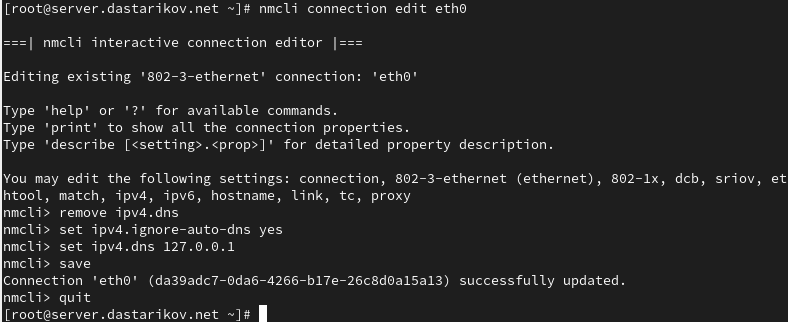
\includegraphics[width=0.8\textwidth]{../images/image04.png}
    \captionof{figure}{Настройка сетевого соединения eth0.}
    \label{04}
\end{center}

    \item Сделали тоже самое для соединения System eth0 (Рис. \ref{04}):
        \begin{minted}{bash}
        nmcli connection edit System\ eth0
        remove ipv4.dns
        set ipv4.ignore-auto-dns yes
        set ipv4.dns 127.0.0.1
        save
        quit
        \end{minted}

\begin{center}
    \centering
    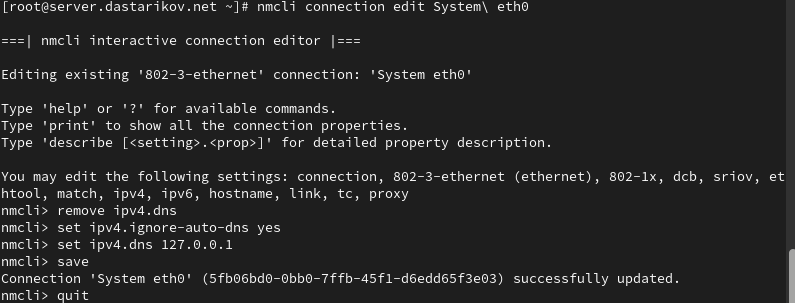
\includegraphics[width=0.8\textwidth]{../images/image05.png}
    \captionof{figure}{Настройка сетевого соединения System eth0.}
    \label{05}
\end{center}

    \item Перезапустили NetworkManager:
        \begin{minted}{bash}
        systemctl restart NetworkManager
        \end{minted}
    Проверили наличие изменений в файле {\tt /etc/resolv.conf}.
    \item Для настройки направления DNS-запросов от всех узлов внутренней сети, включая запросы от узла server, через узел server внесли изменения в файл {\tt /etc/named.conf}, заменив строку
        \begin{minted}{bash}
        listen-on port 53 { 127.0.0.1; };
        \end{minted}
    на
        \begin{minted}{bash}
        listen-on port 53 { 127.0.0.1; any; };
        \end{minted}
    и строку
        \begin{minted}{bash}
        allow-query { localhost; };
        \end{minted}
    на
        \begin{minted}{bash}
        allow-query { localhost; 192.168.0.0/16; };
        \end{minted}
    \item Внесли изменения в настройки межсетевого экрана узла server, разрешив работу с DNS (Рис. \ref{06}):
        \begin{minted}{bash}
        firewall-cmd --add-service=dns
        firewall-cmd --add-service=dns --permanent
        \end{minted}

\begin{center}
    \centering
    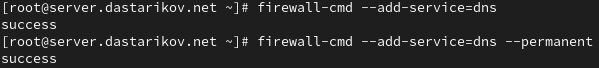
\includegraphics[width=0.8\textwidth]{../images/image06.png}
    \captionof{figure}{Настройка межсетевого экрана.}
    \label{06}
\end{center}

    \item Убедились, что DNS-запросы идут через узел server, который прослушивает порт 53 (Рис. \ref{07}):
        \begin{minted}{bash}
        lsof | grep UDP
        \end{minted}

\begin{center}
    \centering
    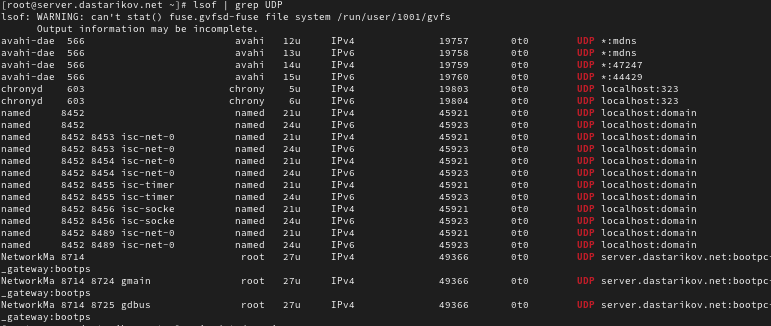
\includegraphics[width=0.8\textwidth]{../images/image07.png}
    \captionof{figure}{Просмотр прослушиваемых портов.}
    \label{07}
\end{center}

\end{enumerate}

\subsubsection{Конфигурирование кэширующего DNS-сервера при наличии фильтрации DNS-запросов маршрутизаторами}
В случае возникновения в сети ситуации, когда DNS-запросы от сервера филь- труются сетевым оборудованием, следует добавить перенаправление DNS-запросов на конкретный вышестоящий DNS-сервер. Для этого в конфигурационный файл {\tt named.conf} в секцию options добавили
        \begin{minted}{bash}
    forwarders { список DNS-серверов };
    forward first;
        \end{minted}
% Текущий список DNS-серверов можно получить, введя на локальном хосте (на котором развёртывается образ виртуальной машины) следующую команду:
Получили список DNS-серверов:
        \begin{minted}{bash}
    cat /etc/resolv.conf
        \end{minted}
% Например, для хостов в дисплейном классе мы получим следующие данные для конфигурационного файла named.conf виртуальной машины server:
%     forwarders { 10.128.0.240; 80.250.174.240; };
%     forward first;
Кроме того, возможно вышестоящий DNS-сервер может не поддерживать технологию DNSSEC, тогда следует в конфигурационном файле {\tt named.conf} указать следующие настройки:
        \begin{minted}{bash}
    dnssec-enable no;
    dnssec-validation no;
        \end{minted}
\subsection{Конфигурирование первичного DNS-сервера}
\begin{enumerate}
     \item Скопировали шаблон описания DNS-зон named.rfc1912.zones из каталога {\tt /etc} в каталог {\tt /etc/named} и переименовали его в dastarikov.net (Рис. \ref{08}):
        \begin{minted}{bash}
        cp /etc/named.rfc1912.zones /etc/named/
        cd /etc/named
        mv /etc/named/named.rfc1912.zones /etc/named/dastarikov.net
        \end{minted}

\begin{center}
    \centering
    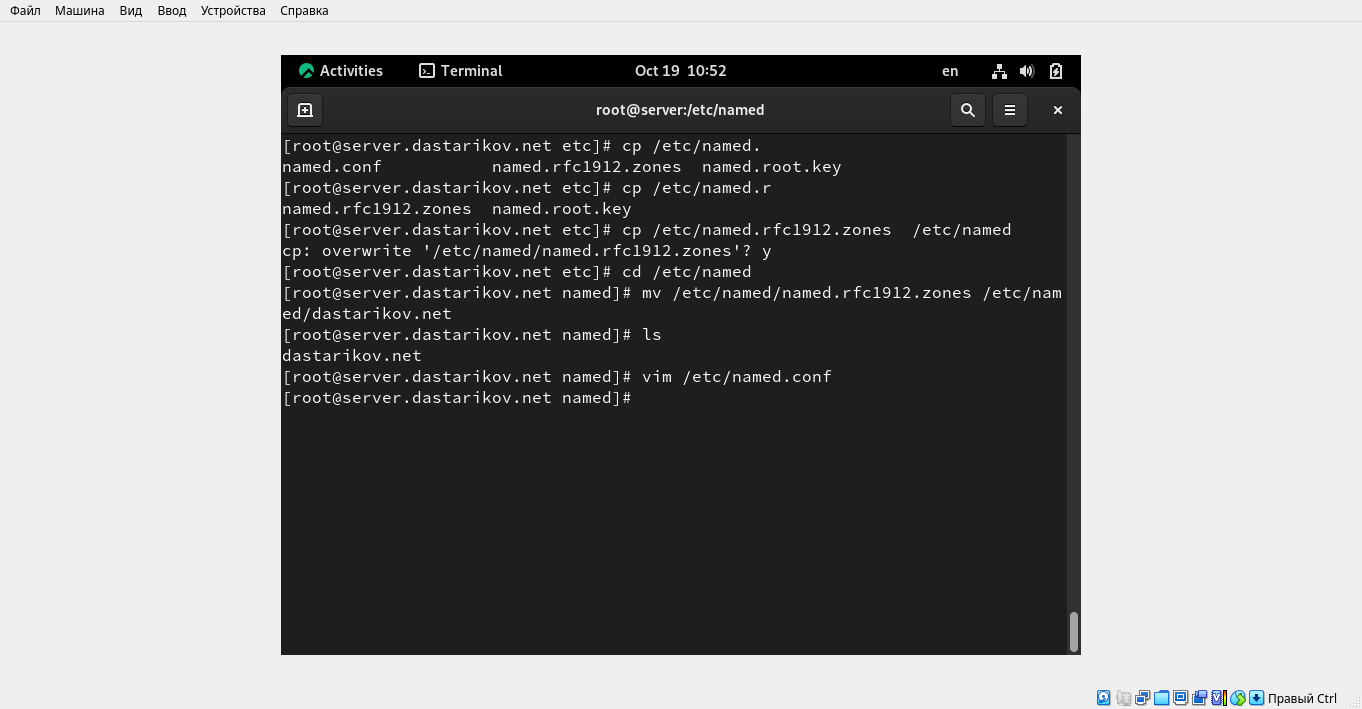
\includegraphics[width=0.8\textwidth]{../images/image08.png}
    \captionof{figure}{Настройка файлов для описания DNS-зон.}
    \label{08}
\end{center}

    \item Включили файл описания зоны {\tt /etc/named/dastarikov.net} в конфигурационном файле DNS /etc/named.conf, добавив в нём в конце строку:
        \begin{minted}{bash}
        include "/etc/named/dastarikov.net";
        \end{minted}
    \item Открыли файл {\tt /etc/named/dastarikov.net} на редактирование и вместо зоны (Рис. \ref{09})
        \begin{minted}{bash}
        zone "localhost.localdomain" IN {
            type master;
            file "named.localhost";
            allow-update { none; };
        };
        \end{minted}
    прописали свою прямую зону:
        \begin{minted}{bash}
        zone "dastarikov.net" IN {
            type master;
            file "master/fz/dastarikov.net";
            allow-update { none; };
        };
        \end{minted}
    Далее, вместо зоны
        \begin{minted}{bash}
        zone "1.0.0.127.in-addr.arpa" IN {
            type master;
            file "named.loopback";
            allow-update { none; };
        };
        \end{minted}
    прописали свою обратную зону (Рис. \ref{09}):
        \begin{minted}{bash}
        zone "1.168.192.in-addr.arpa" IN {
            type master;
            file "master/rz/192.168.1";
            allow-update { none; };
        };
        \end{minted}

\begin{center}
    \centering
    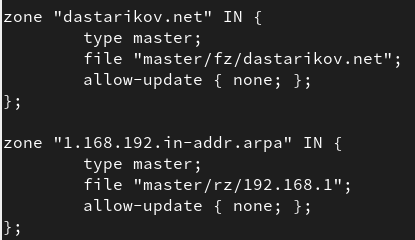
\includegraphics[width=0.8\textwidth]{../images/image09.png}
    \captionof{figure}{Описание DNS-зон.}
    \label{09}
\end{center}

    Остальные записи в файле {\tt /etc/named/dastarikov.net} удалили.
    \item В каталоге {\tt /var/named} создали подкаталоги {\tt master/fz} и {\tt master/rz}, в которых будут располагаться файлы прямой и обратной зоны соответственно:
        \begin{minted}{bash}
        cd /var/named
        mkdir -p /var/named/master/fz
        mkdir -p /var/named/master/rz
        \end{minted}
    \item Скопировали шаблон прямой DNS-зоны named.localhost из каталога {\tt /var/named} в каталог {\tt /var/named/master/fz} и переименовали его в dastarikov.net:
        \begin{minted}{bash}
        cp /var/named/named.localhost /var/named/master/fz/
        cd /var/named/master/fz/
        mv named.localhost dastarikov.net
        \end{minted}
    \item Изменили файл {\tt /var/named/master/fz/dastarikov.net}, указав необходимые DNS-записи для прямой зоны. В этом файле DNS-имя сервера @ rname.invalid. заменили на @ server.dastarikov.net.; формат серийного номера ГГГГММДДВВ (ГГГГ — год, ММ — месяц, ДД — день, ВВ — номер ревизии) [1]; адрес в A-записи заменили с 127.0.0.1 на 192.168.1.1; в директиве \$ORIGIN задали текущее имя домена dastarikov.net., а затем указаны имена и адреса серверов в этом домене в виде A-записей DNS (на данном этапе должен быть прописан сервер с именем ns и адресом 192.168.1.1) (Рис. \ref{10}).
        % При этом внимательно отнеситесь к синтаксису в этом файле, а именно к пробелам и табуляции. В результате должен получиться файл следующего содержания:
        % NOTE: взять из сгенерированного файла
        \begin{minted}{bash}
        $TTL 1D
        @ IN SOA @ server.dastarikov.net. (
        2024072700 ; serial
        1D ; refresh
        1H ; retry
        1W ; expire
        3H ) ; minimum
        NS @
        A 192.168.1.1
        $ORIGIN dastarikov.net.
        server A 192.168.1.1
        ns A 192.168.1.1
\end{minted}

\begin{center}
    \centering
    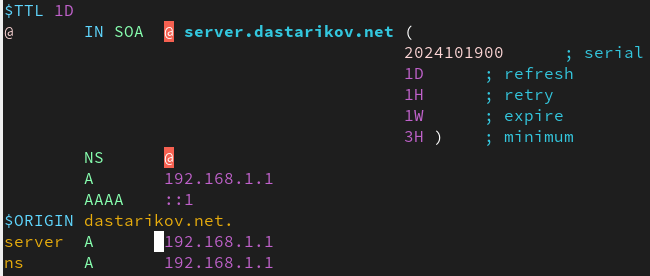
\includegraphics[width=0.8\textwidth]{../images/image10.png}
    \captionof{figure}{Настройка прямой DNS-зоны.}
    \label{10}
\end{center}

    \item Скопировали шаблон обратной DNS-зоны named.loopback из каталога {\tt /var/named} в каталог {\tt /var/named/master/rz} и переименовали его в 192.168.1:
        \begin{minted}{bash}
        cp /var/named/named.loopback /var/named/master/rz/
        cd /var/named/master/rz/
        mv named.loopback 192.168.1
        \end{minted}
    \item Изменили файл {\tt /var/named/master/rz/192.168.1}, указав необходимые DNS-записи для обратной зоны. В этом файле DNS-имя сервера @ rname.invalid. заменили на @ server.dastarikov.net.; формат серийного номера ГГГГММДДВВ (ГГГГ — год, ММ — месяц, ДД — день, ВВ — номер ревизии); адрес в A-записи заменили с 127.0.0.1 на 192.168.1.1; в директиве \$ORIGIN задали название обратной зоны в виде 1.168.192.in-addr.arpa., затем задали PTR-записи (на данном этапе должна быть задана PTR запись, ставящая в соответствие адресу 192.168.1.1 DNS-адрес ns.dastarikov.net). В результате должен получиться файл следующего содержания (Рис. \ref{11}):
        % NOTE: взять из сгенерированного файла
        \begin{minted}{bash}
        $TTL 1D
        @ IN SOA @ server.dastarikov.net. (
        2024072700 ; serial
        1D ; refresh
        1H ; retry
        1W ; expire
        3H ) ; minimum
        NS @
        A 192.168.1.1
        PTR server.dastarikov.net.
        $ORIGIN 1.168.192.in-addr.arpa.
        1 PTR server.dastarikov.net.
        1 PTR ns.dastarikov.net.
        \end{minted}

\begin{center}
    \centering
    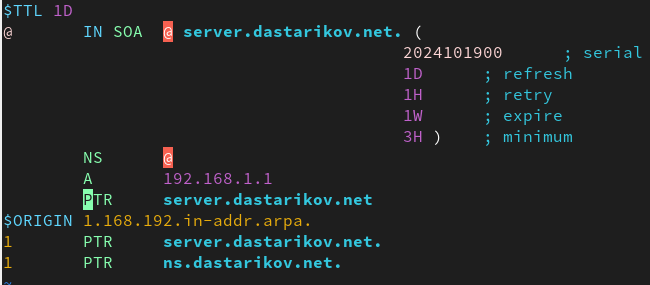
\includegraphics[width=0.8\textwidth]{../images/image11.png}
    \captionof{figure}{Настройка обратной DNS-зоны.}
    \label{11}
\end{center}

    \item Далее исправили права доступа к файлам в каталогах {\tt /etc/named} и {\tt /var/named}, чтобы демон named мог с ними работать (Рис. \ref{12}):
        \begin{minted}{bash}
        chown -R named:named /etc/named
        chown -R named:named /var/named
        \end{minted}
    \item В системах с запущенным SELinux все процессы и файлы имеют специальные метки безопасности (так называемый «контекст безопасности»), используемые системой для принятия решений по доступу к этим процессам и файлам. После изменения доступа к конфигурационным файлам named восстановили их метки в SELinux (Рис. \ref{12}):
        \begin{minted}{bash}
        restorecon -vR /etc
        restorecon -vR /var/named
        \end{minted}
    Для проверки состояния переключателей SELinux, относящихся к named, ввели (Рис. \ref{12}):
        \begin{minted}{bash}
        getsebool -a | grep named
        \end{minted}
    При необходимости дали named разрешение на запись в файлы DNS-зоны (Рис. \ref{12}):
        \begin{minted}{bash}
        setsebool named_write_master_zones 1
        setsebool -P named_write_master_zones 1
        \end{minted}

\begin{center}
    \centering
    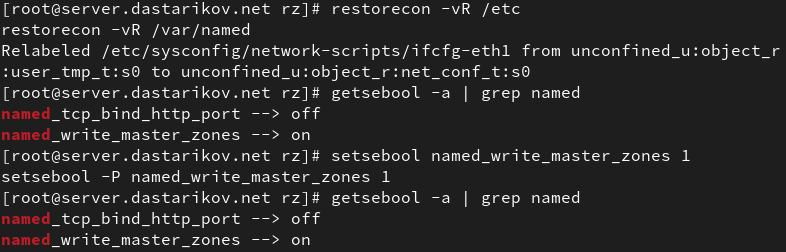
\includegraphics[width=0.8\textwidth]{../images/image12.png}
    \captionof{figure}{Настройка меток SELinux.}
    \label{12}
\end{center}

    \item Во дополнительном терминале запустили в режиме реального времени расширенный лог системных сообщений, чтобы проверить корректность работы системы (Рис. \ref{13}):
        \begin{minted}{bash}
        journalctl -x -f
        \end{minted}
    и в первом терминале перезапустили DNS-сервер:
        \begin{minted}{bash}
        systemctl restart named
        \end{minted}
    % NOTE: Если в логе выдаются сообщения об ошибках, то устраните их и повторно перезапустите DNS-сервер.

\begin{center}
    \centering
    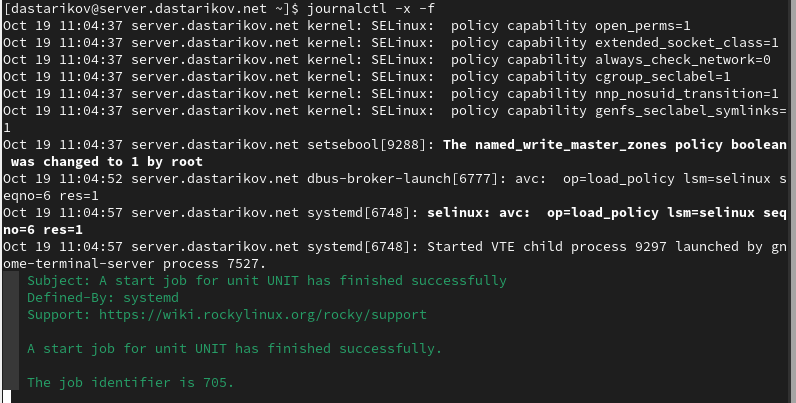
\includegraphics[width=0.8\textwidth]{../images/image13.png}
    \captionof{figure}{Просмотр записей журнала системных сообщений.}
    \label{13}
\end{center}

\end{enumerate}

\subsection{Анализ работы DNS-сервера}
\begin{enumerate}
    \item При помощи утилиты dig получили описание DNS-зоны с сервера {\tt ns.dastarikov.net} (Рис. \ref{14}):
        \begin{minted}{bash}
        dig ns.dastarikov.net
        \end{minted}

\begin{center}
    \centering
    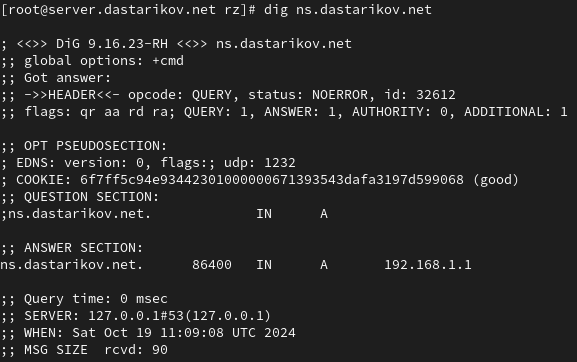
\includegraphics[width=0.8\textwidth]{../images/image14.png}
    \captionof{figure}{Получение описания DNS-зоны с сервара.}
    \label{14}
\end{center}

    \item При помощи утилиты host проанализировали корректность работы DNS-сервера (Рис. \ref{16}):
        \begin{minted}{bash}
        host -l dastarikov.net
        host -a dastarikov.net
        host -t A dastarikov.net
        host -t PTR 192.168.1.1
        \end{minted}

\begin{center}
    \centering
    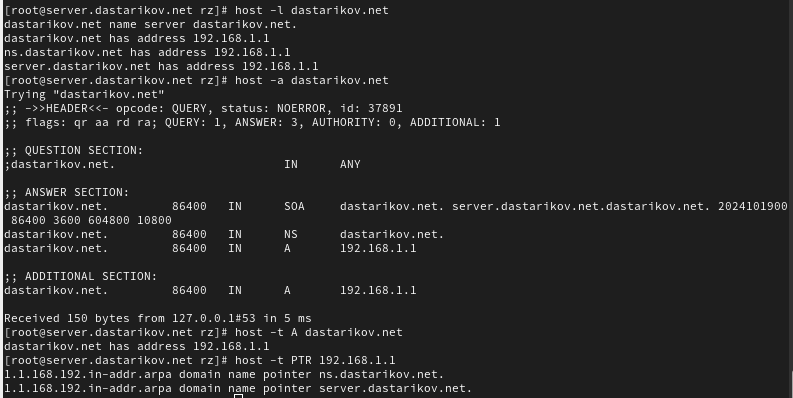
\includegraphics[width=0.8\textwidth]{../images/image16.png}
    \captionof{figure}{Проверка корректиности работы DNS-сервера.}
    \label{16}
\end{center}

\end{enumerate}

\subsection{Внесение изменений в настройки внутреннего окружения виртуальной машины}
\begin{enumerate}
    \item На виртуальной машине server перешли в каталог для внесения изменений в настройки внутреннего окружения {\tt /vagrant/provision/server/}, создайте в нём каталог dns, в который поместили в соответствующие каталоги конфигурационные файлы DNS:
        \begin{minted}{bash}
        cd /vagrant
        mkdir -p /vagrant/provision/server/dns/etc/named
        mkdir -p /vagrant/provision/server/dns/var/named/master/
        cp -R /etc/named.conf /vagrant/provision/server/dns/etc/
        cp -R /etc/named/* /vagrant/provision/server/dns/etc/named/
        cp -R /var/named/master/* /vagrant/provision/server/dns/var/named/master/
        \end{minted}
    \item В каталоге {\tt /vagrant/provision/server} создали исполняемый файл {\tt dns.sh}:
        \begin{minted}{bash}
        touch dns.sh
        chmod +x dns.sh
        \end{minted}
        Открыв его на редактирование, прописали в нём следующий скрипт:
        \begin{minted}{bash}
        #!/bin/bash
        echo "Provisioning script $0"
        echo "Install needed packages"
        dnf -y install bind bind-utils
        echo "Copy configuration files"
        cp -R /vagrant/provision/server/dns/etc/* /etc
        cp -R /vagrant/provision/server/dns/var/named/* /var/named
        chown -R named:named /etc/named
        chown -R named:named /var/named
        restorecon -vR /etc
        restorecon -vR /var/named
        echo "Configure firewall"
        firewall-cmd --add-service=dns
        firewall-cmd --add-service=dns --permanent
        echo "Tuning SELinux"
        setsebool named_write_master_zones 1
        setsebool -P named_write_master_zones 1
        echo "Change dns server address"
        nmcli connection edit "System eth0" <<EOF
        remove ipv4.dns
        set ipv4.ignore-auto-dns yes
        set ipv4.dns 127.0.0.1
        save
        quit
        EOF
        systemctl restart NetworkManager
        echo "Start named service"
        systemctl enable named
        systemctl start named
        \end{minted}
    \item Для отработки созданного скрипта во время загрузки виртуальной машины server в конфигурационном файле Vagrantfile добавили в разделе конфигурации для сервера:
        \begin{minted}{bash}
        server.vm.provision "server dns",
        type: "shell",
        preserve_order: true,
        path: "provision/server/dns.sh"
        \end{minted}
\end{enumerate}
\section{Выводы}
В результате лабораторной работы приобрели практические навыки по установке и конфигурированию DNS-сервера.

\end{document}
